\section{Argon Molecular Dynamics}

We can now apply these statistical ideas to the results of your argon MD simulation. Run as
long a simulation as is practical and make measurements of the temperature, potential energy
and the time average of the virial, which is given by
%
\begin{equation}
    \sum_i \sum_{j > i} r_{ij} \frac{ \partial V_{ij} }{ \partial r_{ij} }
\end{equation}
%
every MD time step. You should be able to run a few thousand steps, after thermalization.


\Question{} Measure the autocorrelation times for the temperature, potential energy and
virial.

\Answer{}
We run the Argon molecular dynamics from the last homework for a total \(24046\) steps,
and after \(15000\) steps we reached desired temperature (around \(1.0718\)).
Therefore, there are \(9047\) total steps for doing a statistical analysis.

We plot the potential energy, kinetic energy, and total energy in Figure~\ref{fig:MD_e_t},
which corresponds to the simulation time from \(t = 480\) to \(770\).

\begin{figure}[hb]
    \centering
    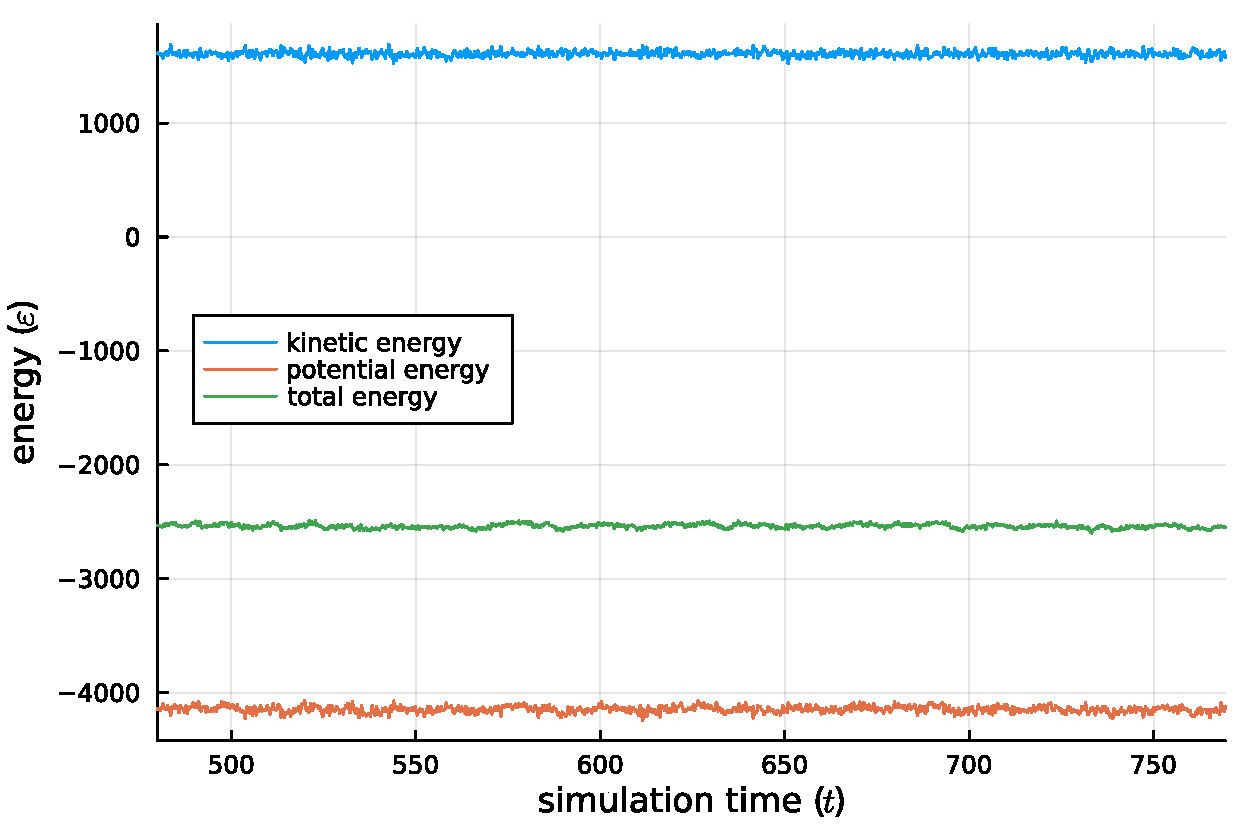
\includegraphics[width=0.8\textwidth]{e-t}
    \caption{The potential energy, kinetic energy, and total energy for the
        Argon molecular dynamics from simulation time from \(t = 480\) to \(770\).}
    \label{fig:MD_e_t}
\end{figure}

The temperature and virial terms are plotted in
Figure~\ref{fig:MD:a} and Figure~\ref{fig:MD:b}, respectively.

\begin{figure}[H]
    \centering
    \begin{minipage}[t]{0.8\linewidth}
        \centering
        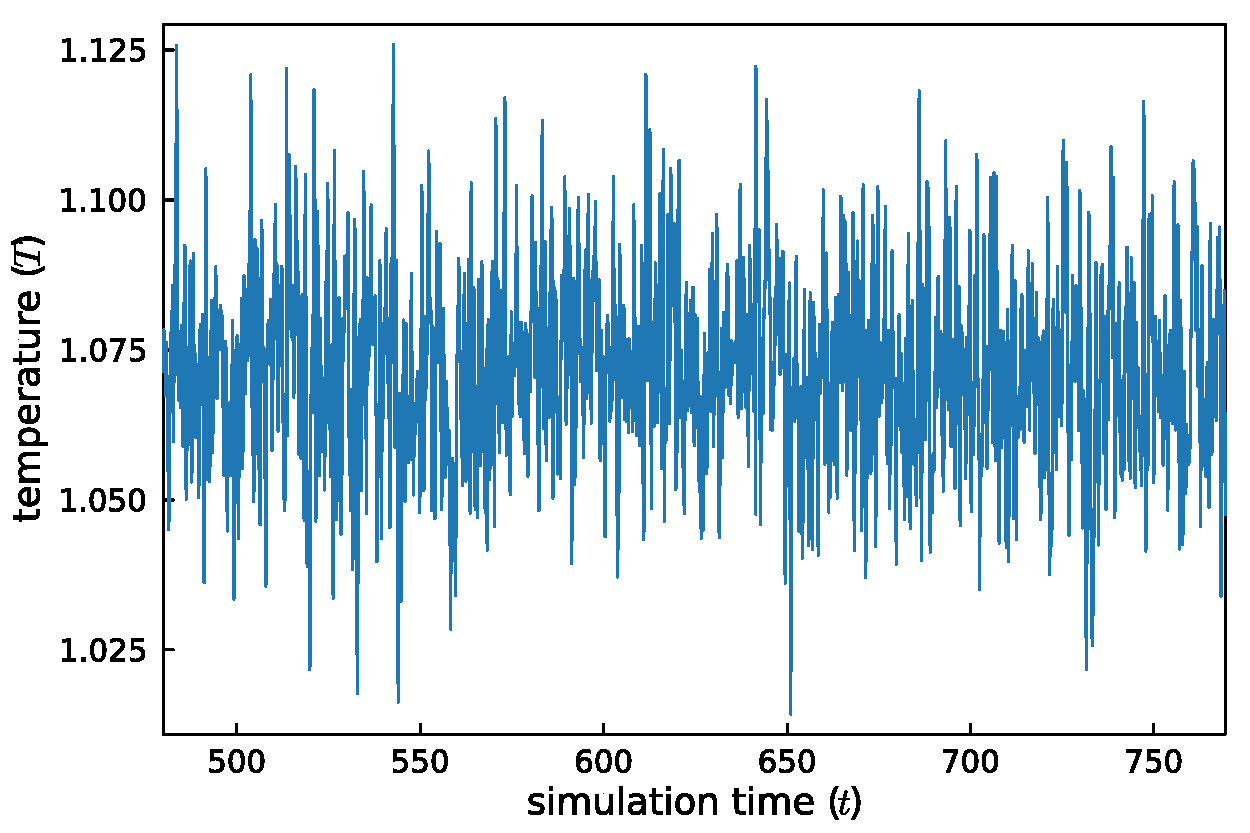
\includegraphics[width=\linewidth]{MD_temperature}
        \subcaption{The temperature for the
            Argon molecular dynamics from simulation time from \(t = 480\) to \(770\).}
        \label{fig:MD:a}
    \end{minipage}
    \hfill
    \begin{minipage}[t]{0.8\linewidth}
        \centering
        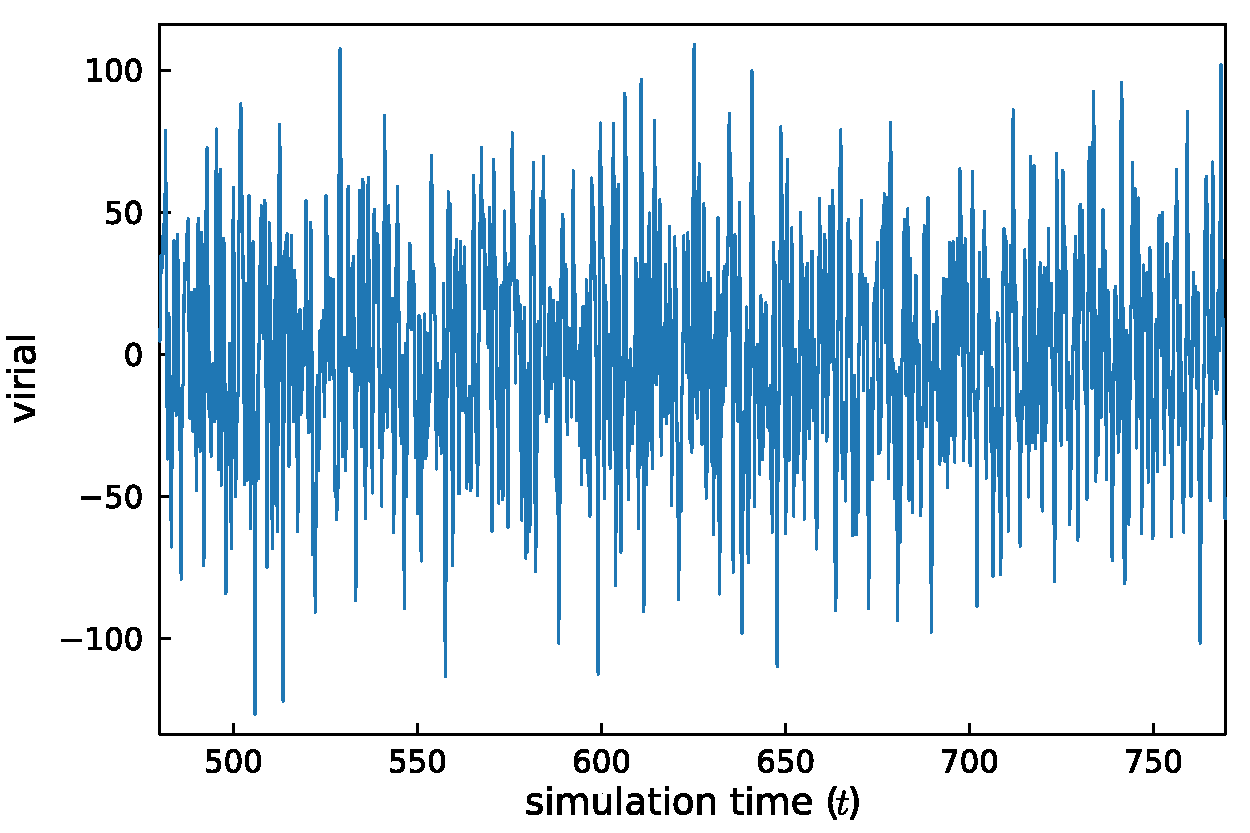
\includegraphics[width=\linewidth]{MD_virial}
        \subcaption{The virial for the
            Argon molecular dynamics from simulation time from \(t = 480\) to \(770\).}
        \label{fig:MD:b}
    \end{minipage}
    \caption{The temperature and virial terms for the
        Argon molecular dynamics.}
    \label{fig:MD}
\end{figure}

Similar to Problem~\ref{sec:ja}, we plot the integrated autocorrelation time
for temperature, potential energy, and virial as functions of \(n_\textnormal{cut}\)
in Figures~\ref{fig:MD_iat:a},
\ref{fig:MD_iat:b}, and~\ref{fig:MD_iat:c}.
As we can see, they are all short compared to the total number of time steps,
this is because we have a relative small number of total steps, similar to
Problem~\ref{sec:mock}.

\begin{figure}
    \centering
    \begin{minipage}[t]{0.8\linewidth}
        \centering
        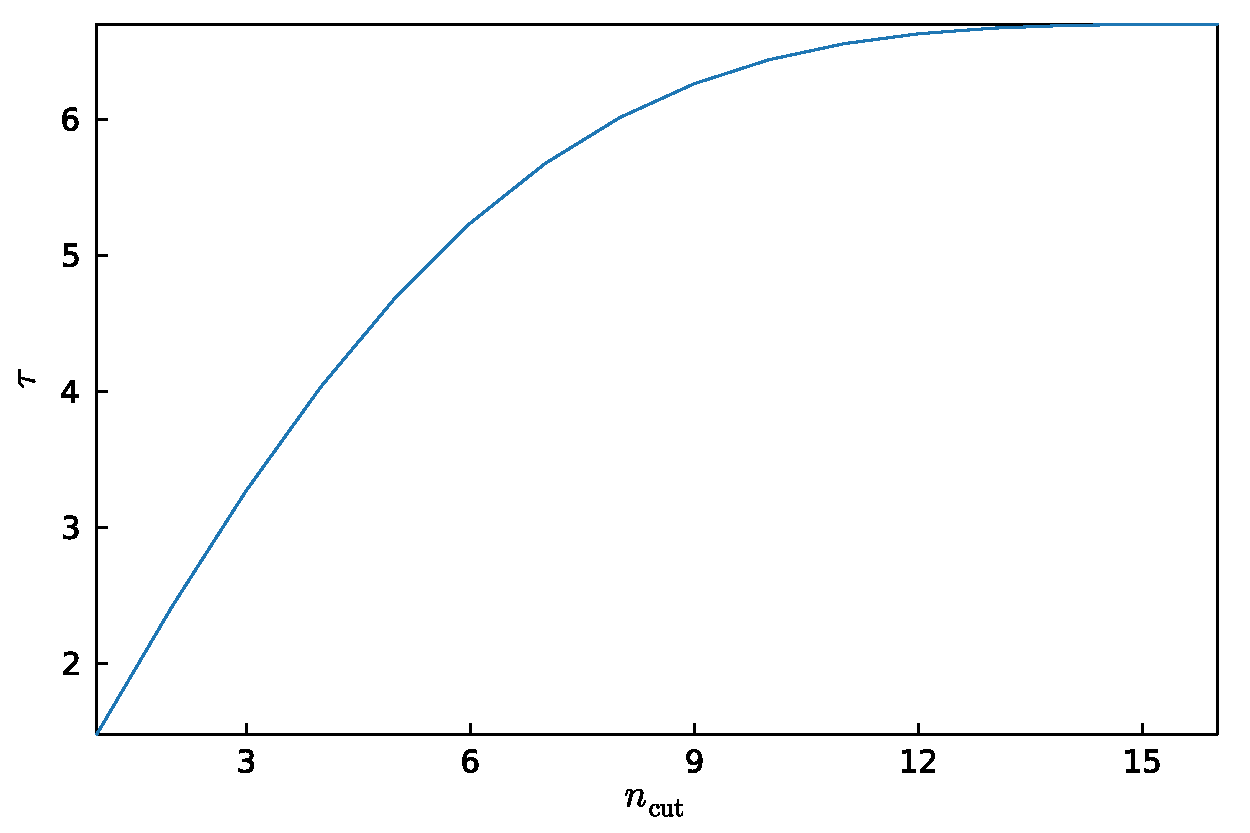
\includegraphics[width=\linewidth]{MD_tau_temperature}
        \subcaption{The integrated autocorrelation time for temperature.}
        \label{fig:MD_iat:a}
    \end{minipage}
    \hfill
    \begin{minipage}[t]{0.8\linewidth}
        \centering
        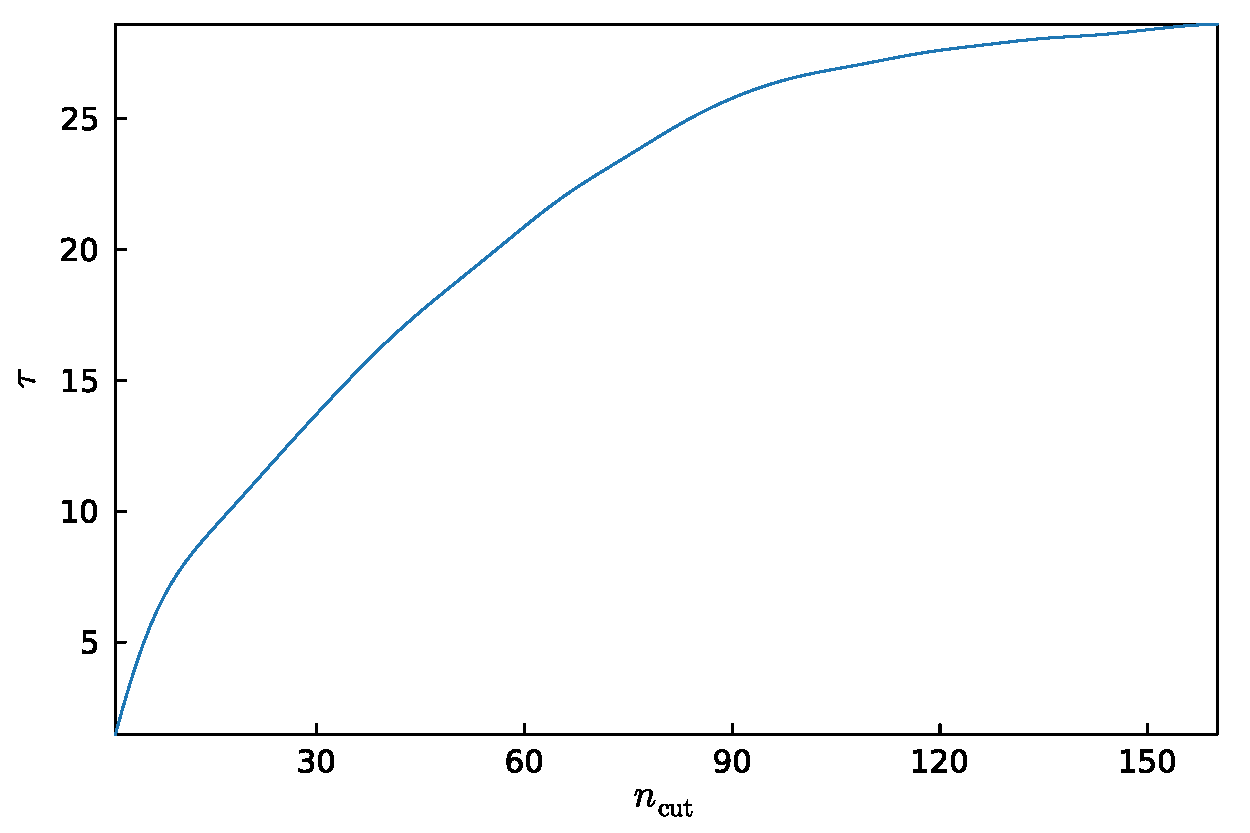
\includegraphics[width=\linewidth]{MD_tau_energy}
        \subcaption{The integrated autocorrelation time for the potential energy.}
        \label{fig:MD_iat:b}
    \end{minipage}
    \caption{The integrated autocorrelation time for temperature and the potential energy.}
    \label{fig:MD_iat}
\end{figure}

\begin{figure}[H]
    \centering
    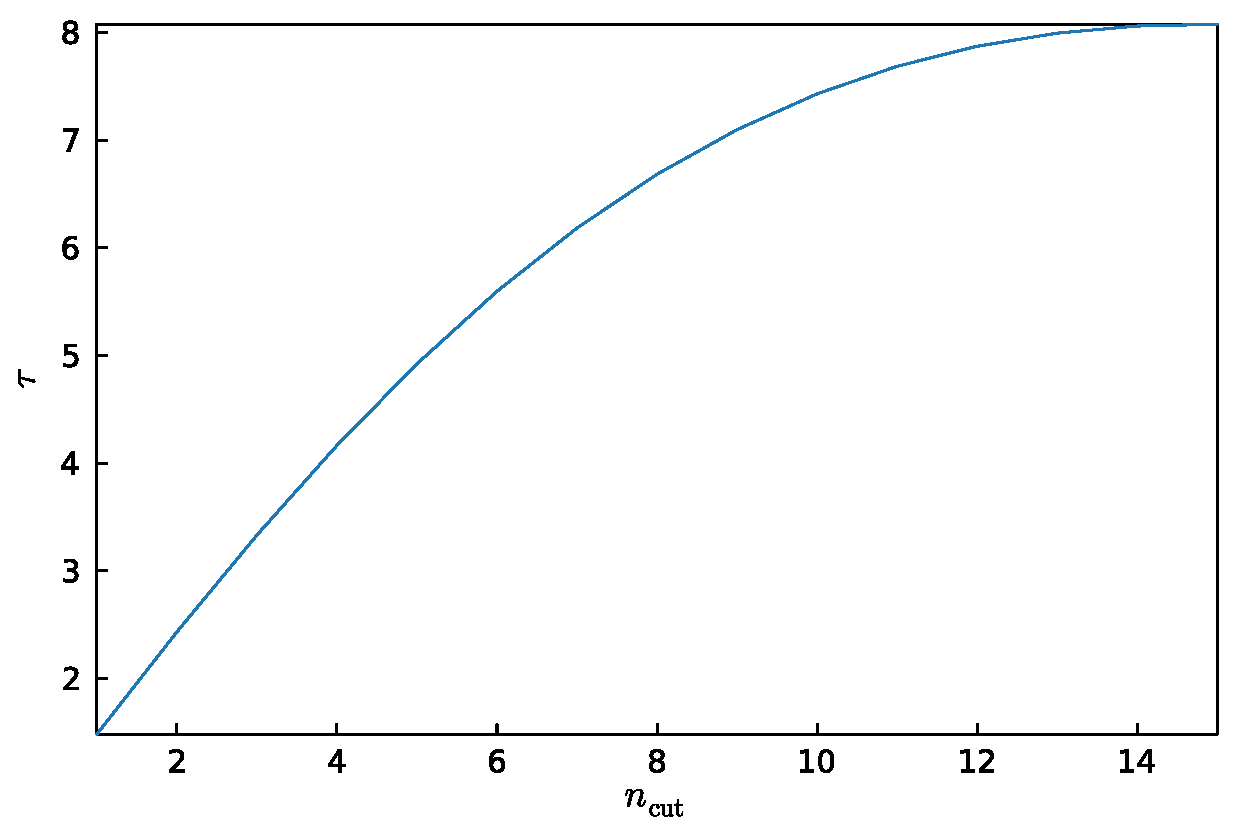
\includegraphics[width=0.8\textwidth]{MD_tau_virial}
    \caption{The integrated autocorrelation time for the virial.}
    \label{fig:MD_iat:c}
\end{figure}


\Question{} Also measure the covariance matrix for these \(3\) quantities.

\Answer{}
The covariance matrix for temperature, potential energy, and virial is
%
\begin{equation}
    \hat{c} =
    \begin{bmatrix}
        0.00024  & -0.30849  & 0.00425    \\
        -0.30849 & 698.43424 & 84.42649   \\
        0.00425  & 84.42649  & 1296.32289
    \end{bmatrix}.
\end{equation}
%
And the normalized version of the covariance is
%
\begin{equation}
    \hat{\rho} =
    \begin{bmatrix}
        1        & -0.75095 & 0.00759 \\
        -0.75095 & 1        & 0.08873 \\
        0.00759  & 0.08873  & 1
    \end{bmatrix}.
\end{equation}
%
As we can see, the temperature and potential energy are negatively correlated.
This is understandable since the total energy is fixed, and the potential energy and
the kinetic energy are negatively correlated, while the temperature and the kinetic
energy are positively correlated.
And the temperature and the virial are positive correlated since the kinetic energy
and the virial satisfy the following relation:
%
\begin{equation}
    \langle T \rangle = \frac{ 1 }{ 2 }
    \sum_i
    \biggl\langle r_i \frac{ \partial U }{ \partial r_i } \biggr\rangle.
\end{equation}


\Question{} Use your estimate of the autocorrelation times, along with binning and the
jackknife method to give an error on the pressure from your simulation.

\Answer{}

